

\subsection{Miscellaneous Options}
\label{pgfplots:misc}

\begin{pgfplotskey}{disablelogfilter=\mchoice{true,false} (initally false, default true)}
Disables numerical evaluation of $\log(x)$ in \TeX. If you specify this option, any plot coordinates and tick positions must be provided as $\log(x)$ instead of $x$. This may be faster and -- possibly -- more accurate than the numerical log. The current implementation of $\log(x)$ normalizes~$x$ to $m\cdot 10^e$ and computes
\[ \log(x) = \log(m) + e \log(10) \]
where $y = \log(m)$ is computed with a newton method applied to $\exp(y) - m$. The normalization involves string parsing without \TeX-registers. You can savely evaluate $\log(1\cdot 10^{-7})$ although \TeX-registers would produce an underflow for such small numbers. 
\end{pgfplotskey}

\label{sec:disabledatascaling}%
\begin{pgfplotskey}{disabledatascaling=\mchoice{true,false} (initally false, default true)}
\index{Accuracy!Data Transformation}%
\index{Errors!dimension too large}%
Disables internal re-scaling of input data. Normally, every input data like plot coordinates, tick positions or whatever, are parsed without using \TeX's limited number precision. Then, a transformation like 
	\[ T(x) = 10^{q-m} \cdot x - a \]
is applied to every input coordinate/position where $m$ is ``the order of $x$'' base~$10$. Example: $x=1234 = 1.234\cdot 10^3$ has order~$m=4$ while $x=0.001234 = 1.234\cdot 10^{-3}$ has order $m=-2$. The parameter~$q$ is the order of the axis' width/height.

The \textbf{effect} of the transformation is that your plot coordinates can be of \emph{arbitrary magnitude} like $0.0000001$ and $0.0000004$. For these two coordinates, \PGFPlots\ will use 100pt and 400pt internally. The transformation is quit fast since it relies only on period shifts. This scaling allows precision beyond \TeX's capabilities.
%\footnote{Please note that while plot coordinates can be of quite large magnitude like $10^12$ or $10^{-9}$, \PGFPlots\ still uses \TeX-registers internally (the math parser of \PGF). If your axis interval is $[1234567.8, 1234567.9]$ or something like that, }.

The option ``|disabledatascaling|'' disables this data transformation. This has two consequences: first, coordinate expressions like \parg{{\normalfont\texttt{axis cs:}}x,y} have the same effect like \parg{x,y}, no re-scaling is applied. Second, coordinates are restricted to what \TeX\ can handle\footnote{Please note that the axis' scaling requires to compute $1/( x_\text{max} - x_{\text{min}} )$. The option \protect\pgfmanualpdfref{disabledatascaling}{\texttt{disabledatascaling}} may lead to overflow or underflow in this context, so use it with care! Normally, the data scale transformation avoids this problem.}.

So far, the data scale transformation applies only to normal axis (logarithmic scales do not need it). 
\end{pgfplotskey}


\begin{pgfplotsxycodekeylist}{\x\ filter,filter point}
The code keys |x filter| and |y filter| allow coordinate filtering which are based on a \emph{single} coordinate. A coordinate filter gets an input coordinate as |#1|, applies some operation and writes the result into the macro |\pgfmathresult|. If |\pgfmathresult| is empty afterwards, the coordinate is discarded. You can also set |\pgfmathresult| to |nan| or |inf| in which case the coordinate can be either discarded (if |unbounded coords=discard| is set) or the plot can be interrupted (the case |unbounded coords=jump|).

The |filter point/.code| filter allows filtering dependend on all components forming a complete point ($x$, $y$ and $z$); it is described below.

It is allowed if filters do not change |\pgfmathresult|. In this case, the unfiltered coordinate will be used.

Coordinate filters are useful in automatic processing system, where \PGFPlots\ is used to display automatically generated plots. You may not want to filter your coordinates by hand, so these options provide a tool to do this automatically.

The following filter adds $0.5$ to every $x$ coordinate.
\begin{codeexample}[]
\begin{tikzpicture}
\begin{axis}[x filter/.code=
	{\pgfmathadd{#1}{0.5}}]
\addplot coordinates {
	(4,0)
	(6,1)
};
\end{axis}
\end{tikzpicture}
\end{codeexample}
Please refer to~\cite[pgfmath manual]{tikz} for details about the math engine of \PGF. Please keep in mind that the math engine works with limited \TeX\ precision.

During evaluation of the filter, the macro |\coordindex| contains the number of the current coordinate (starting with~$0$). Thus, the following filter discards all coordinates after the $5$th and before the $10$th.
\begin{codeexample}[]
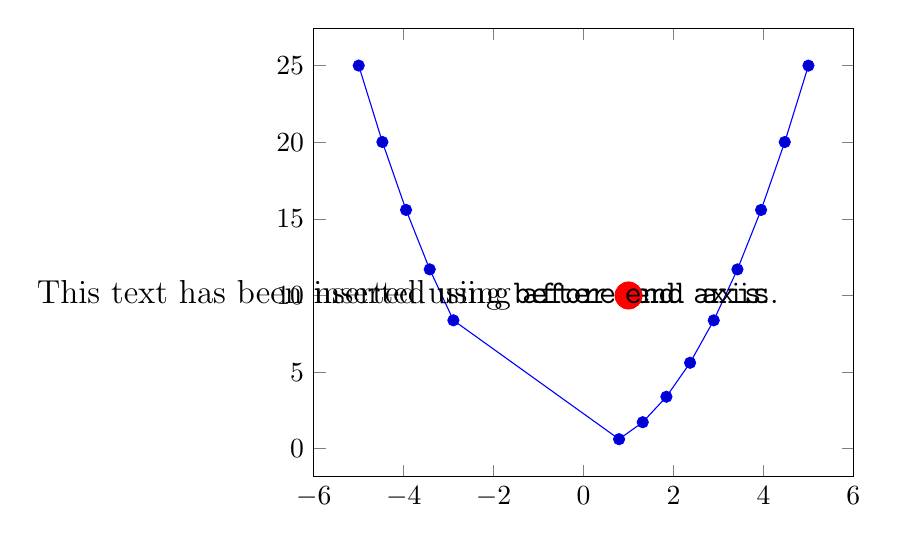
\begin{tikzpicture}
\begin{axis}[
	samples=20,
	x filter/.code={
		\ifnum\coordindex>4
			\ifnum\coordindex<11
				\def\pgfmathresult{}
			\fi
		\fi
	}]
\addplot {x^2};
\end{axis}
\end{tikzpicture}
\end{codeexample}
There is also a style key which simplifies selection by index, see below.

	\PGFPlots\ invokes the filter with argument |#1| set to the input coordinate. For $x$-filters, this is the $x$-coordinate as it is specified to |\addplot|, for $y$-filters it is the $y$-coordinate.

	If the corresponding axis is logarithmic, |#1| is the \emph{logarithm} of the coordinate as a real number, for example |#1=4.2341|.

	The arguments to coordinate filters are usually as they have been found in the input data (i.e.\ no transformation or number parsing has been done at this stage). The ``usually'' has two exceptions: first, for logarithmic axes, the \emph{log} of the argument is supplied.  Second, any high level coordinate maps like |x coord trafo| (which may be used to map dates to numbers or string to numbers or so) are applied. In consequence, the |#1| argument is supposed to be a number.

	If key filters are invoked for |plot table|, access to the current row's data can be achieved using |\thisrow|\marg{column name} (and its variants). This includes all columns of the table.

	The |filter point| key is more technical. It doesn't take an argument: its arguments are given in terms of the |pgfkeys| variables |/data point x|, |/data point y| and |/data point z|. It may change its coordinates using |\pgfkeyssetvalue{/data point x}|\marg{the new value}; access to variables can be get with |\pgfkeysvalueof{/data point/x}| or, if the argument shall be written into a macro, with |\pgfkeysgetvalue|. This filter is evaluated after the other ones.
\end{pgfplotsxycodekeylist}

\begin{stylekey}{/pgfplots/skip coords between index=\marg{begin}\marg{end}}
	A style which appends an |x filter| which discards selected coordinates. The selection is done by index where indexing starts with~$0$, see |\coordindex|. Every coordinate with index $\meta{begin} \le i < \meta{end}$ will be skipped.
\begin{codeexample}[]
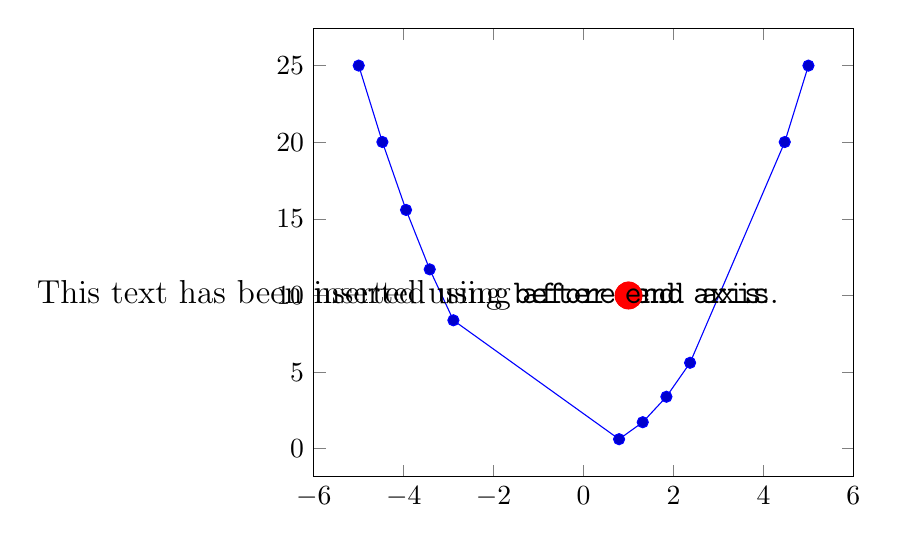
\begin{tikzpicture}
\begin{axis}[
	samples=20,
	skip coords between index={5}{11},
	skip coords between index={15}{18}]

\addplot {x^2};
\end{axis}
\end{tikzpicture}
\end{codeexample}
\end{stylekey}

\begin{pgfplotskey}{each nth point=\marg{integer}}
	A style which appends an |x filter| which discards all but each $n$th input coordinate.
\index{Downsampling}
\end{pgfplotskey}

\begin{pgfplotsxykey}{restrict \x\space to domain=\meta{min}:\meta{max}}
\label{key:restrict:x:to:domain}
	Appends $x$ (or $y$ or $z$) coordinate filters which set the respective coordinate to |-inf| if it is below \meta{min} and to |+inf| if it is above \meta{max}.

	Furthermore, it sets the |unbounded coords=jump| key which leads to interrupted plots.
\begin{codeexample}[]
\begin{tikzpicture}
\begin{axis}[
	restrict y to domain=-10:10,
	samples=1000,
	% some fine tuning for the display:
	width=10cm, height=210pt,
	xmin=-4.7124, xmax=4.7124,
	xtick={-4.7124,-1.5708,...,10},
	xticklabels={$-\frac32 \pi$,$-\pi/2$,$\pi/2$,$\frac32 \pi$},
	axis x line=center,
	axis y line=center]

\addplot[blue] gnuplot[id=tangens,domain=-1.5*pi:1.5*pi] {tan(x)};
\legend{$\tan(x)$}
\end{axis}
\end{tikzpicture}
\end{codeexample}
\end{pgfplotsxykey}

\begin{pgfplotskey}{restrict expr to domain=\marg{expression}\marg{\meta{min}:\meta{max}}}
	Appends an $x$ coordinate filter which sets the $x$ coordinate to |-inf| if the \meta{expression} evaluates to something less than \meta{min} and to |inf| if \meta{expression} evaluates to something larger than \meta{max}.

	Furthermore, it sets the |unbounded coords=jump| key which leads to interrupted plots.

	In contrast to |restrict x to domain|, \meta{expression} can depend on anything which is valid during |\addplot|, in particular |\coordindex| or table columns (|\thisrow|\marg{column name} and friends). The expression doesn't need to depend on $x$ at all.
\end{pgfplotskey}

\begin{pgfplotskey}{filter discard warning=\mchoice{true,false} (initially true)}
	Issues a notification in your logfile whenever coordinate filters discard coordinates.
\end{pgfplotskey}

\begin{pgfplotskey}{execute at begin plot=\marg{commands}}
This axis option allows to invoke \marg{commands} at the beginning of each |\addplot| command. The argument \marg{commands} can be any \TeX\ content.

You may use this in conjunction with |x filter=...| to reset any counters or whatever. An example would be to change every $4$th coordinate.
\end{pgfplotskey}

\begin{pgfplotskey}{execute at end plot=\marg{commands}}
This axis option allows to invoke \marg{commands} after each |\addplot| command. The argument \marg{commands} can be any \TeX\ content.
\end{pgfplotskey}

\begin{pgfplotskey}{forget plot=\marg{true,false} (initially false)}
\label{pgfplots:forgetplot}
	Allows to include plots which are not remembered for legend entries, which do not increase the number of plots and which are not considered for cycle lists.

	A forgotten plot can be some sort of decoration which has a separate style and does not influence the axis state, although it is processed as any other plot.
	Provide this option to |\addplot| as in the following example.
\begin{codeexample}[]
\begin{tikzpicture}
	\begin{loglogaxis}[
		table/x=Basis,
		table/y={L2/r},
		xlabel=Degrees of Freedom,
		ylabel=relative Error,
		title=New Experiments (old in gray),
		legend entries={$e_1$,$e_2$,$e_3$}
	]
	\addplot[black!15,forget plot] 
		table {plotdata/oldexperiment1.dat};
	\addplot[black!15,forget plot] 
		table {plotdata/oldexperiment2.dat};
	\addplot[black!15,forget plot] 
		table {plotdata/oldexperiment3.dat};
	\addplot table {plotdata/newexperiment1.dat};
	\addplot table {plotdata/newexperiment2.dat};
	\addplot table {plotdata/newexperiment3.dat};
	\end{loglogaxis}
\end{tikzpicture}
\end{codeexample}
	Since forgotten plots won't increase the plot index, they will use the same |cycle list| entry as following plots. This can be used to ``interrupt'' plots as is described in section~\ref{pgfplots:interrupt}.
\index{Interrupted Plots}

	The style |every forget plot| can be used to configure styles for each such plot. Please note that |every plot no |\meta{index} styles are not applicable here.

	A forgotten plot will be stacked normally if |stack plots| is enabled!
\end{pgfplotskey}

\begin{pgfplotscodekey}{before end axis}
Allows to insert \marg{commands} just before the axis is ended. This option takes effect inside of the clipped area.
\begin{codeexample}[]
\pgfplotsset{every axis/.append style={
	before end axis/.code={
		\fill[red] (axis cs:1,10) circle(5pt);
		\node at (axis cs:-4,10) 
			{\large This text has been inserted 
			 using \texttt{before end axis}.};
	}}}
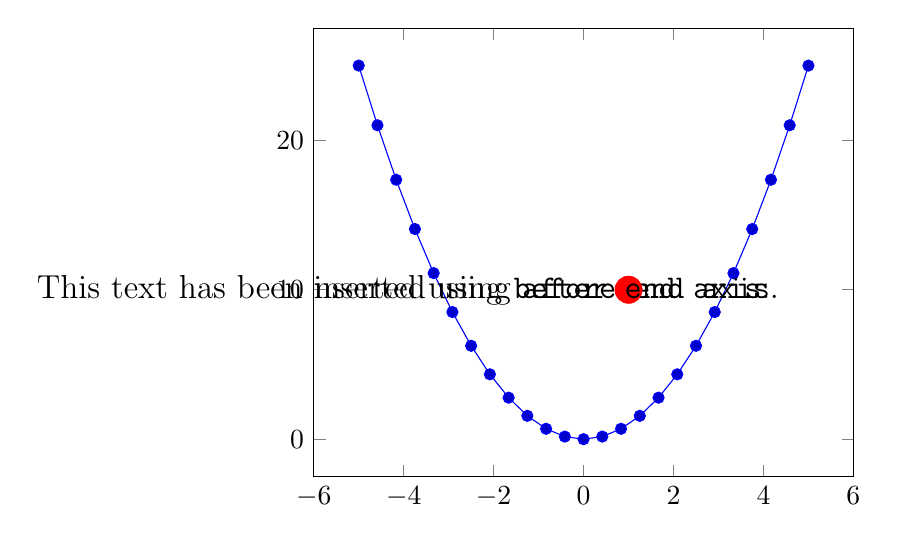
\begin{tikzpicture}
	\begin{axis}
	\addplot {x^2};
	\end{axis}
\end{tikzpicture}
\end{codeexample}
\end{pgfplotscodekey}

\begin{pgfplotscodekey}{after end axis}
Allows to insert \marg{commands} right after the end of the clipped drawing commands. While |befor end axis| has the same effect as if \marg{commands} had been placed inside of your axis, |after end axis| allows to access axis coordinates without being clipped.
\begin{codeexample}[]
\pgfplotsset{every axis/.append style={
	after end axis/.code={
		\fill[red] (axis cs:1,10) circle(5pt);
		\node at (axis cs:-4,10) 
			{\large This text has been inserted using \texttt{after end axis}.};
	}}}
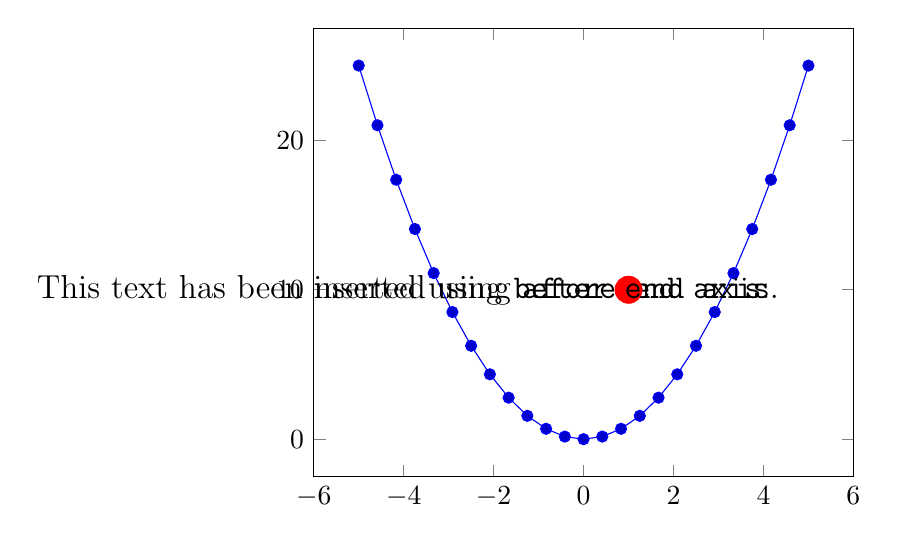
\begin{tikzpicture}
	\begin{axis}
	\addplot {x^2};
	\end{axis}
\end{tikzpicture}
\end{codeexample}
\end{pgfplotscodekey}

\begin{pgfplotskeylist}{nodes near coords=\marg{content of nodes} (default |\textbackslash pgfmathprintnumber\textbackslash pgfplotspointmeta|),
	nodes near coords*=\marg{content of nodes}}
	A style which places nodes near every coordinate.

	This is often used for bar plots, see |ybar| for an example of |nodes near coords|.

	Currently this does not work satisfactory for |ybar interval| or |xbar interval|, sorry.
\end{pgfplotskeylist}

\begin{stylekey}{/pgfplots/every node near coord}
	A style used for every node generated by |nodes near coords|.
\end{stylekey}

\begin{pgfplotskey}{nodes near coords align=\marg{alignment method} (initially auto)}
	Specifies how to align nodes generated by |nodes near coords|. 

	Possible choices for \marg{alignment} are

	\begin{description}
		\item[]\declare{auto} Uses |horizontal| if the $x$ coordinates are shown or |vertical| in all other cases. This checks the current value of |point meta|.
		\item[]\declare{horizontal} uses |left| if |\pgfplotspointmeta| $<0$ and |right| otherwise.
		\item[]\declare{vertical}   uses |below| if |\pgfplotspointmeta| $<0$ and |above| otherwise.
		\item[any \Tikz\ alignment option] such as |anchor=north east|, |below| or something like that. It is also allowed if multiple options are provided.
	\end{description}
\end{pgfplotskey}

\begin{pgfplotskey}{clip marker paths=\mchoice{true,false} (initially false)}
	The initial choice |clip marker paths=false| causes markers to be drawn \emph{after} the clipped region. Only their positions will be clipped. As a consequence, markers will be drawn completely, or not at all. The value |clip marker paths=true| is here for backwards compatibility: it does not introduce special marker treatment, so markers may be drawn partially if they are close to the clipping boundary\footnote{Please note that clipped marker paths may be slightly faster during \TeX\ compilation.}.
\end{pgfplotskey}

\begin{pgfplotskey}{clip=\mchoice{true,false} (initially true)}
	Whether any paths inside an axis shall be clipped.
\end{pgfplotskey}

\begin{pgfplotskey}{axis on top=\mchoice{true,false} (initially false)}
	If set to |true|, axis lines, ticks, tick labels and grid lines will be drawn on top of plot graphics.
\begin{codeexample}[]
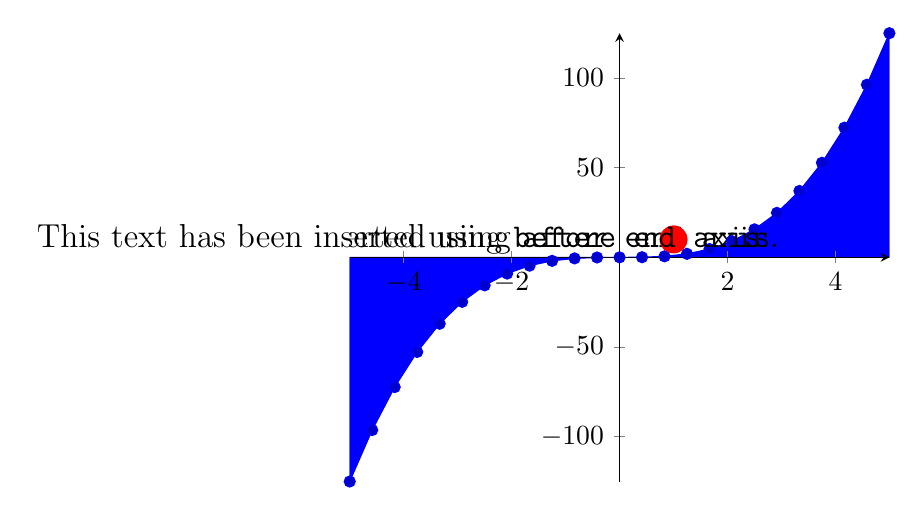
\begin{tikzpicture}
    \begin{axis}[
		axis on top=true,
		axis x line=middle,
		axis y line=middle]
    \addplot+[fill] {x^3} \closedcycle;
    \end{axis}
\end{tikzpicture}
\end{codeexample}

\begin{codeexample}[]
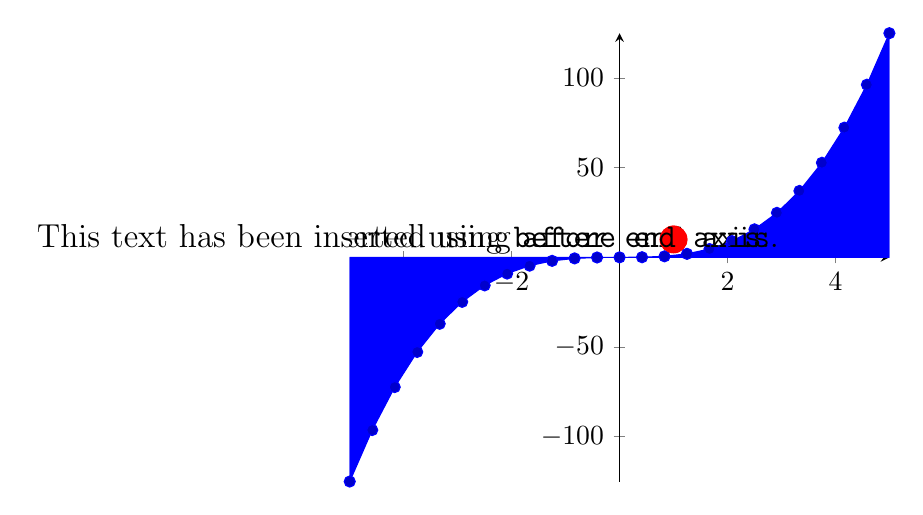
\begin{tikzpicture}
    \begin{axis}[
		axis on top=false,
		axis x line=middle,
		axis y line=middle]
    \addplot+[fill] {x^3} \closedcycle;
    \end{axis}
\end{tikzpicture}
\end{codeexample}
Please note that this feature does not affect plot marks. I think it looks unfamiliar if plot marks are crossed by axis descriptions.
\end{pgfplotskey}

\begin{key}{/pgf/fpu=\marg{true,false} (initially true)}
\index{Precision}
	This key activates or deactivates the floating point unit. If it is disabled (|false|), the core \PGF\ math engine written by Mark Wibrow and Till Tantau will be used for |plot expression|.
	However, this engine has been written to produce graphics and is not suitable for scientific computing. It is limited to fixed point numbers in the range $\pm 16384.00000$.

	If the |fpu| is enabled (|true|, the initial configuration) the high-precision floating point library of \PGF\ written by Christian Feuers\"anger will be used. It offers the full range of IEEE double precision computing in \TeX. This FPU is also part of \PGFPlotstable, and it is activated by default for |create col/expr| and all other predefined mathematical methods.

	Use
\begin{codeexample}[code only]
\pgfkeys{/pgf/fpu=false}
\end{codeexample}
	\noindent in order to de-activate the extended precision. If you prefer using the |fp| (fixed point) package, possibly combined with Mark Wibrows corresponding \PGF\ library, the |fpu| will be deactivated automatically. Please note, however, that |fp| has a smaller data range (about $\pm 10^{17}$) and may be slower.
\end{key}

\subsection{Miscellaneous Commands}
\begin{command}{\autoplotspeclist}
This command should no longer be used, although it will be kept as technical implementation detail. Please use the `|cycle list|' option, section~\ref{sec:cycle:list}.
\end{command}

\begin{command}{\pgfmathlogtologten\meta{number}}
Assigns the result of $\meta{number}/\log(10)$ to |\pgfmathresult|.
\end{command}

\begin{command}{\logten}
Expands to the constant $\log(10)$. Useful for logplots because $\log(10^i) = i\log(10)$. This command is only available inside of an \Tikz-picture.
\end{command}

\begin{command}{\pgfmathprintnumber\marg{number}}
Generates pretty--printed output\footnote{This method was previously \texttt{\textbackslash prettyprintnumber}. It's functionality has been included into \PGF\ and the old command is now deprecated.} for \marg{number}. This method is used for every tick label.

The number is printed using the current number printing options, see section~\ref{sec:number:printing} for the different number styles, rounding precision and rounding methods.
\end{command}

\begin{command}{\plotnum}
	Inside of |\addplot| or any associated style, option or command, |\plotnum| expands to the current plot's number, starting with~$0$.
\end{command}

\begin{command}{\numplots}
	Inside of any of the axis environments, associated style, option or command, |\numplots| expands to the total number of  plots.
\end{command}

\begin{command}{\coordindex}
	Inside of an |\addplot| command, this macro expands to the number of the actual coordinate (starting with~$0$).

	It is useful together with |x filter| or |y filter| to (de-)select coordinates.
\end{command}

\begin{command}{\pgfplotstableread\marg{file}}
	Please refer to the manual of \PGFPlotstable, |pgfplotstable.pdf|, which is part of the \PGFPlots-bundle.
\end{command}
\begin{command}{\pgfplotstabletypeset\marg{\textbackslash macro}}
	Please refer to the manual of \PGFPlotstable, |pgfplotstable.pdf|, which is part of the \PGFPlots-bundle.
\end{command}
